\section{Model} \label{sec:model}
\begin{figure*}[t]
	\begin{subfigure}[b]{0.292\linewidth}
		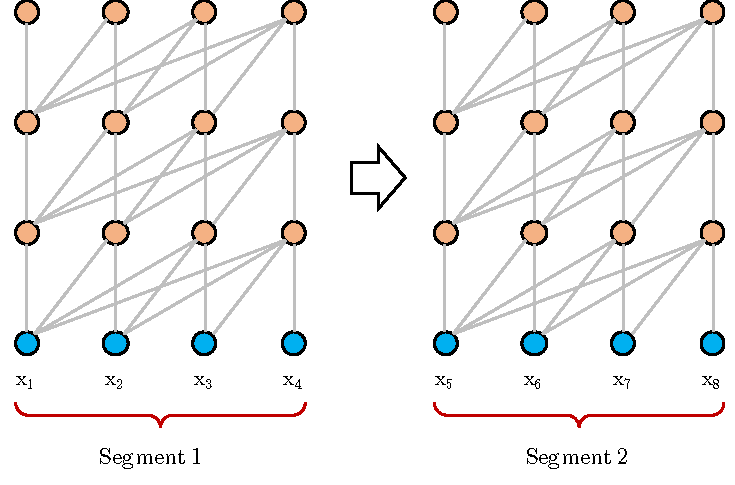
\includegraphics[width=\textwidth]{FIG/vanilla-train.pdf}
		\caption{\small Train phase.}
		\label{fig:vanilla-train}
	\end{subfigure}
	\rulesep
	\begin{subfigure}[b]{0.69\linewidth}
		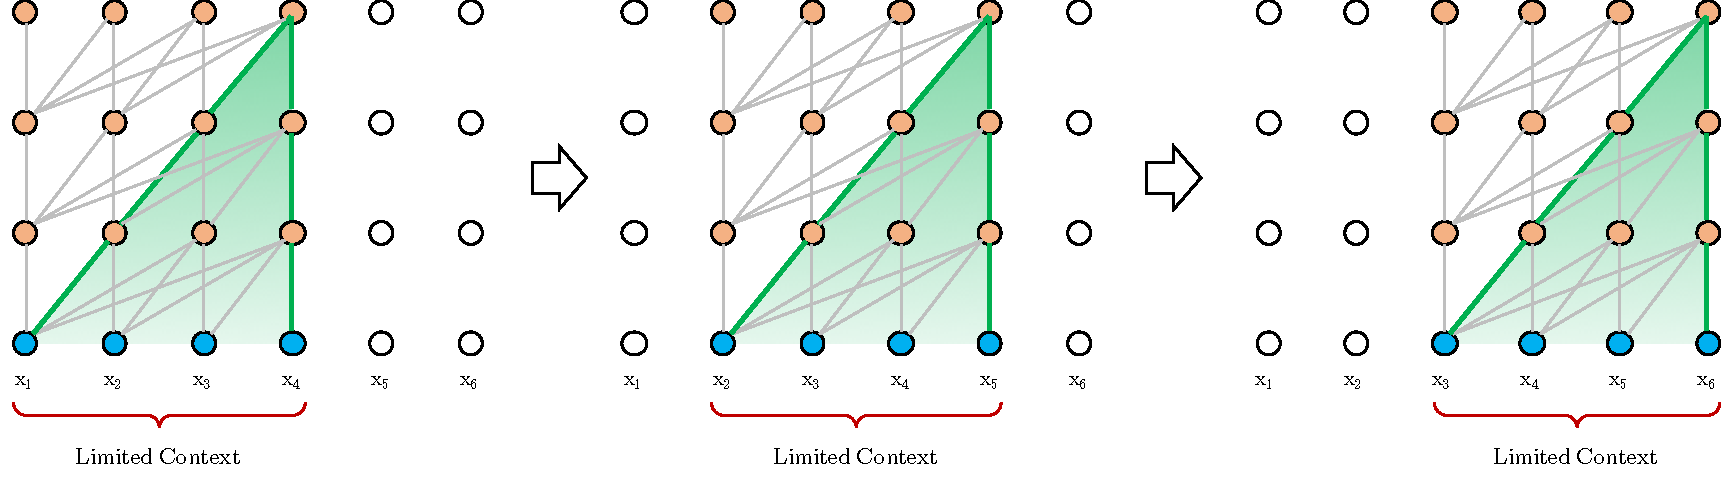
\includegraphics[width=\textwidth]{FIG/vanilla-eval.pdf}
		\caption{\small Evaluation phase.}
		\label{fig:vanilla-eval}
	\end{subfigure}
	\caption{\small Illustration of the vanilla model with a segment length 4.}
	\label{fig:vanilla}
\vspace{-1em}
\end{figure*}

Given a corpus of tokens $\rvx = (x_1 , \dots, x_T)$, the task of language modeling is to estimate the joint probability $P(\rvx)$, which is often auto-regressively factorized as $P(\rvx) = \prod_{t} P(x_t \mid \rvx_{<t})$.
With the factorization, the problem reduces to estimating each conditional factor.
In this work, we stick to the standard neural approach to modeling the conditional probability.
Specifically, a trainable neural network is used to encode the context $\rvx_{<t}$ into a fixed size hidden state, which is multiplied with the word embeddings to obtain the logits.
The logits are then fed into the Softmax function, yielding a categorical probability distribution over the next token.

\subsection{Vanilla Transformer Language Models}
In order to apply Transformer or self-attention to language modeling, the central problem is how to train a Transformer to effectively encode an arbitrarily long context into a fixed size representation.
% that can lead to a good estimation of the conditional probability.
Given infinite memory and computation, a simple solution would be to process the entire context sequence using an unconditional Transformer decoder, similar to a feed-forward neural network.
% , and train the network with gradient descent.
However, this is usually infeasible with the limited resource in practice.


One feasible but crude approximation is to split the entire corpus into shorter segments of manageable sizes, and only train the model within each segment, ignoring all contextual information from previous segments.
% This is exactly the idea adapted by~\citet{al2018character}, which we refer to as the \textit{vanilla model} and visualize in Fig. \ref{fig:vanilla-train}.
This is the idea adopted by \citet{al2018character}. We call it the \textit{vanilla model} and visualize it in Fig. \ref{fig:vanilla-train}.
Under this training paradigm, information never flows across segments in either the forward or backward pass.
% , no matter it is the forward or backward pass.
There are two critical limitations of using a fixed-length context.
First, the largest possible dependency length is upper bounded by the segment length, which is a few hundred on character-level language modeling \citep{al2018character}.
Therefore, although the self-attention mechanism is less affected by the vanishing gradient problem compared to RNNs, the vanilla model is not able to fully exploit this optimization advantage.
Second, though it is possible to use padding to respect the sentence or other semantic boundaries, in practice it has been standard practice to simply chunk long text into fixed-length segments due to improved efficiency \citep{peters2018deep,devlin2018bert,al2018character}. However, simply chunking a sequence into fixed-length segments will lead to the context fragmentation problem as discussed in Section \ref{sec:intro}.

During evaluation, at each step, the vanilla model also consumes a segment of the same length as in training, but only makes one prediction at the last position.
Then, at the next step, the segment is shifted to the right by only one position, and the new segment has to be processed all from scratch.
As shown in Fig.~\ref{fig:vanilla-eval}, this procedure ensures that each prediction utilizes the longest possible context exposed during training, and also relieves context fragmentation issue encountered in training. However, this evaluation procedure is extremely expensive. We will show that our proposed architecture is able to substantially improve the evaluation speed.

\subsection{Segment-Level Recurrence with State Reuse}

% While the capacity of the vanilla model is limited by segment-based training, a related segment-based approximation was proposed for RNN training called the \textit{truncated back-propagation through time} (BPTT)~\citep{mikolov2010recurrent}.
% In truncated BPTT, the last RNN hidden state of the previous segment is passed to the next segment as a \textit{fixed} input in the forward pass.
% Although the gradient still remains within a segment, this additional input allows the RNN to exploit information in the history, leading to an ability of modeling longer-term dependency~\citep{khandelwal2018sharp}.


% The only difference lies in that,
% the information encoded in the hidden state passed from the last segment, leading to a potentially longer context.
% In practice, this technique has proven to be very successful, allowing RNN-LMs to capture much longer dependency than the length of a training segment.

\begin{figure*}[!h]
	\begin{subfigure}[b]{0.62\linewidth}
		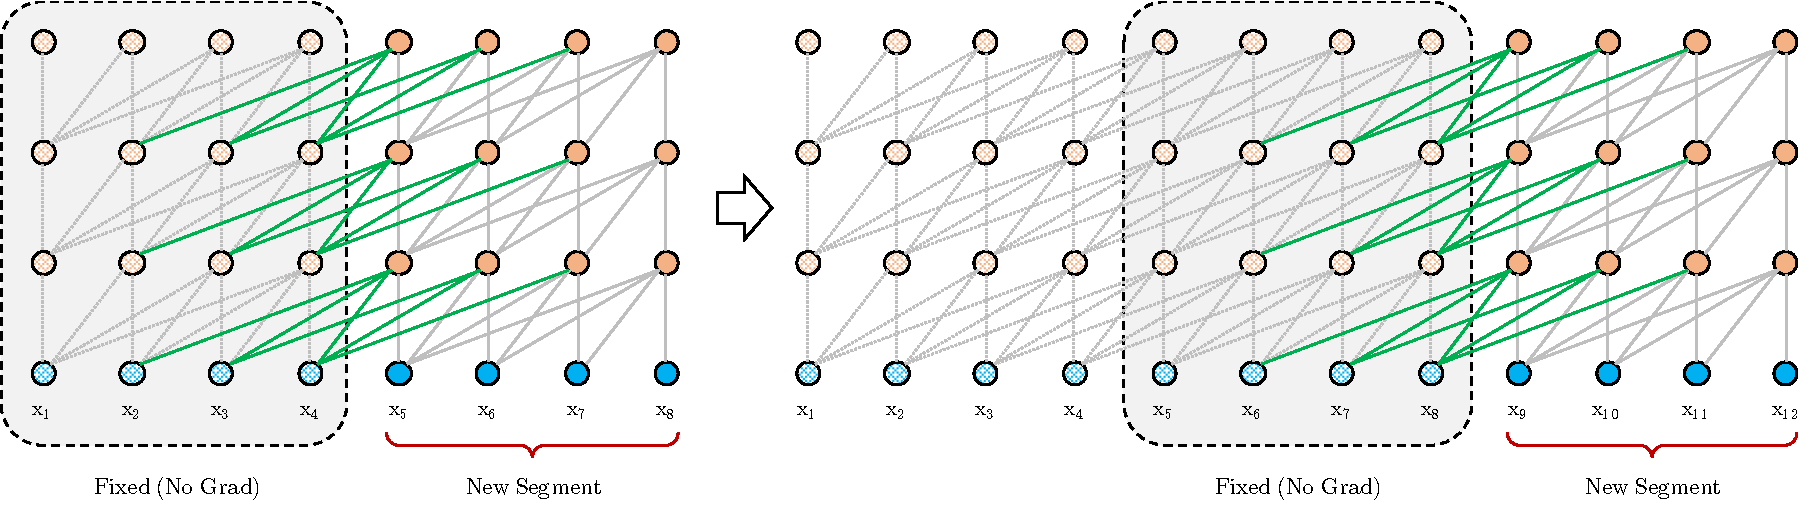
\includegraphics[width=\textwidth]{FIG/xl-train.pdf}
		\caption{\small Training phase.}
		\label{fig:xl-train}
	\end{subfigure}
	\rulesep
	\begin{subfigure}[b]{0.35\linewidth}
		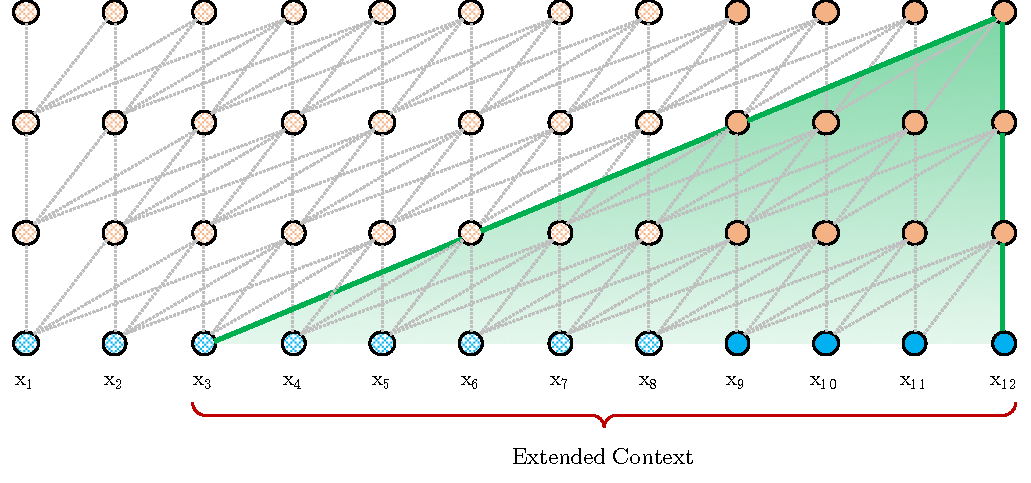
\includegraphics[width=\textwidth]{FIG/xl-eval.pdf}
		\caption{\small Evaluation phase.}
		\label{fig:xl-eval}
	\end{subfigure}
	\caption{\small Illustration of the Transformer-XL model with a segment length 4.}
	\label{fig:xl}
\vspace{-1em}
\end{figure*}
To address the limitations of using a fixed-length context, we propose to introduce a recurrence mechanism to the Transformer architecture.
During training, the hidden state sequence computed for the previous segment is \textit{fixed} and \textit{cached} to be reused as an extended context when the model processes the next new segment, as shown in Fig. \ref{fig:xl-train}.
Although the gradient still remains within a segment, this additional input allows the network to exploit information in the history, leading to an ability of modeling longer-term dependency and avoiding context fragmentation.
Formally, let the two consecutive segments of length $L$ be $\rvs_{\tau} = \left[x_{\tau,1}, \cdots, x_{\tau,L}\right]$ and $\rvs_{\tau+1} = \left[x_{\tau+1,1}, \cdots, x_{\tau+1,L}\right]$ respectively.
Denoting the $n$-th layer hidden state sequence produced for the $\tau$-th segment $\rvs_{\tau}$ by $\rvh_{\tau}^{n} \in \R^{L \times d}$, where $d$ is the hidden dimension.
Then, the $n$-th layer hidden state for segment $\rvs_{\tau+1}$ is produced (schematically) as follows,
\par\nobreak
\vspace{-0.5em}
\small
\begin{align*}\label{eqn:reuse}
	&\widetilde{\rvh}_{\tau+1}^{n-1} = \left[ \text{SG}(\rvh_{\tau}^{n-1}) \circ \rvh_{\tau+1}^{n-1} \right],
%		&& \text{(extended context)} 
		\\
	&\rvq_{\tau+1}^{n}, \rvk_{\tau+1}^{n}, \rvv_{\tau+1}^{n} = \rvh_{\tau+1}^{n-1} \rmW_q^\top, \widetilde{\rvh}_{\tau+1}^{n-1} \rmW_k^\top, \widetilde{\rvh}_{\tau+1}^{n-1} \rmW_v^\top,
%		&& \text{(query, key, value vectors)} 
		\\
	&\rvh_{\tau+1}^{n} = \text{Transformer-Layer}\left(\rvq_{\tau+1}^{n}, \rvk_{\tau+1}^{n}, \rvv_{\tau+1}^{n}\right).
%		&& \text{(self-attention + feed-forward)}
\end{align*}
\normalsize
\vspace{-1.5em}

\noindent where the function $\text{SG}(\cdot)$ stands for stop-gradient, the notation $[\rvh_u \circ \rvh_v]$ indicates the concatenation of two hidden sequences along the length dimension, and $\mathbf{W}_\cdot$ denotes model parameters.
Compared to the standard Transformer, the critical difference lies in that the key $\rvk_{\tau+1}^{n}$ and value $\rvv_{\tau+1}^{n}$ are conditioned on the extended context $\widetilde{\rvh}_{\tau+1}^{n-1}$ and hence $\rvh_{\tau}^{n-1}$ cached from the previous segment.
We emphasize this particular design by the green paths in Fig. \ref{fig:xl-train}.

With this recurrence mechanism applied to every two consecutive segments of a corpus, it essentially creates a segment-level recurrence in the hidden states.
As a result, the effective context being utilized can go way beyond just two segments.
However, notice that the recurrent dependency between $\rvh_{\tau+1}^{n}$ and $\rvh_{\tau}^{n-1}$ shifts one layer downwards per-segment, which differs from the same-layer recurrence in conventional RNN-LMs.
Consequently, the largest possible dependency length grows linearly w.r.t. the number of layers as well as the segment length, i.e., $O(N \times L)$, as visualized by the shaded area in Fig. \ref{fig:xl-eval}.
% Although the context information is still finite in theory, it can be easily extended to infinite by further employing the depth-wise recurrence as in \citep{dehghani2018universal}.
This is analogous to truncated BPTT \citep{mikolov2010recurrent}, a technique developed for training RNN-LMs. However, different from truncated BPTT, our method caches a sequence of hidden states instead of the last one, and should be applied together with the relative positional encoding technique described in Section \ref{sec:rel-pos-embed}.

Besides achieving extra long context and resolving fragmentation, another benefit that comes with the recurrence scheme is significantly faster evaluation.
Specifically, during evaluation, the representations from the previous segments can be reused instead of being computed from scratch as in the case of the vanilla model.
In our experiments on enwiki8, Transformer-XL is up to 1,800+ times faster than the vanilla model during evaluation (see Section \ref{sec:exp}).

% the representation of the context sequence does not have to be recomputed from scratch as in the case of the vanilla model.
% Instead, the previously computed hidden representations can be directly reused to produce the states of the new inputs.

Finally, notice that the recurrence scheme does not need to be restricted to only the previous segment.
In theory, we can cache as many previous segments as the GPU memory allows, and reuse all of them as the extra context when processing the current segment.
% However, as the model parameter changes consistently during training, the hidden states previously computed using old parameters are inevitably stale, which may make the optimization difficult.
% In practice, we didn't observe any significant problem of this sort.
Thus, we can cache a predefined length-$M$ old hidden states spanning (possibly) multiple segments, and refer to them as the memory $\rvm_{\tau}^{n} \in \R^{M \times d}$, due to a clear connection to the memory augmented neural networks~\citep{graves2014neural,weston2014memory}.
In our experiments, we set $M$ equal to the segment length during training, and increase it by multiple times during evaluation.


\subsection{Relative Positional Encodings}
\label{sec:rel-pos-embed}
While we found the idea presented in the previous subsection very appealing, there is a crucial technical challenge we haven't solved in order to reuse the hidden states.
That is, how can we keep the positional information coherent when we reuse the states?
Recall that, in the standard Transformer, the information of sequence order is provided by a set of positional encodings, denoted as $\rmU \in \R^{L_\text{max} \times d}$, where the $i$-th row $\rmU_i$ corresponds to the $i$-th \textit{absolute} position within a segment and $L_\text{max}$ prescribes the maximum possible length to be modeled.
Then, the actual input to the Transformer is the element-wise addition of the word embeddings and the positional encodings.
If we simply adapt this positional encoding to our recurrence mechanism, the hidden state sequence would be computed schematically by
\par\nobreak
\vspace{-0.5em}
\small
\begin{align*}
	\rvh_{\tau+1} &= f(\rvh_{\tau}, \rmE_{\rvs_{\tau+1}} + \rmU_{1:L}) \\
	\rvh_{\tau} &= f(\rvh_{\tau-1}, \rmE_{\rvs_{\tau}} + \rmU_{1:L}),
\end{align*}
\normalsize
\vspace{-1.5em}
%\[
%	\rvh_{\tau+1} = f(\rvh_{\tau}, \rmE_{\rvs_{\tau+1}} + \rmU_{1:L}) \quad\text{and}\quad \rvh_{\tau} = f(\rvh_{\tau-1}, \rmE_{\rvs_{\tau}} + \rmU_{1:L}),
%\]

\noindent where $\rmE_{\rvs_{\tau}} \in \R^{L \times d}$ is the word embedding sequence of $\rvs_{\tau}$, and $f$ represents a transformation function.
Notice that, both $\rmE_{\rvs_{\tau}}$ and $\rmE_{\rvs_{\tau+1}}$ are associated with the same positional encoding $\rmU_{1:L}$.
As a result, the model has no information to distinguish the positional difference between $x_{\tau,j}$ and $x_{\tau+1,j}$ for any $j = 1, \dots, L$, resulting in a sheer performance loss.

In order to avoid this failure mode, the fundamental idea is to only encode the \textit{relative} positional information in the hidden states.
Conceptually, the positional encoding gives the model a temporal clue or ``bias'' about how information should be gathered, i.e., where to attend.
For the same purpose, instead of incorporating bias statically into the initial embedding, one can inject the same information into the attention score of each layer.
More importantly, it is more intuitive and generalizable to define the temporal bias in a relative manner.
For instance, when a query vector $q_{\tau,i}$ attends on the key vectors $\rvk_{\tau,\leq i}$, it does not need to know the absolute position of each key vector to identify the temporal order of the segment.
Instead, it suffices to know the relative distance between each key vector $k_{\tau,j}$ and itself $q_{\tau,i}$, i.e. $i - j$. %\footnote{In this work, as we focus on language modeling, the attention is also causal, i.e., from right to left. Hence, the relative distance, defined as the right index minus the left index, is always non-negative. But it is straightforward to extend this idea to the non-causal case.}
Practically, one can create a set of relative positional encodings $\rmR \in \R^{L_\text{max} \times d}$, where the $i$-th row $\rmR_i$ indicates a relative distance of $i$ between two positions.
By injecting the relative distance dynamically into the attention score, the query vector can easily distinguish the representations of $x_{\tau,j}$ and $x_{\tau+1,j}$ from their different distances, making the state reuse mechanism feasible.
Meanwhile, we won't lose any temporal information, as the absolute position can be recovered recursively from relative distances.

Previously, the idea of relative positional encodings has been explored in the context of machine translation~\citep{shaw2018self} and music generation~\citep{huang2018improved}.
Here, we offer a different derivation, arriving at a new form of relative positional encodings, which not only has a one-to-one correspondence to its absolute counterpart but also enjoys much better generalization empirically (see Section \ref{sec:exp}).
Firstly, in the standard Transformer \citep{vaswani2017attention}, the attention score between query $q_i$ and key vector $k_j$ within the same segment can be decomposed as
\par\nobreak
\vspace{-0.5em}
\small
\begin{align*}
	\rmA_{i,j}^\text{abs} %= q_i^\top k_j
	&= \underbrace{ \rmE_{x_i}^\top \rmW_q^\top \rmW_k \rmE_{x_j} }_{(a)}
	+ \underbrace{\rmE_{x_i}^\top \rmW_q^\top \rmW_k \rmU_{j}}_{(b)} \\
	&+ \underbrace{\rmU_{i}^\top \rmW_q^\top \rmW_k \rmE_{x_j}}_{(c)}
	+ \underbrace{\rmU_{i}^\top \rmW_q^\top \rmW_k \rmU_{j}}_{(d)}. \vspace{-0.5em}
\end{align*}
\normalsize
\vspace{-1em}

Following the idea of only relying on relative positional information, we propose to re-parameterize the four terms as follows
\par\nobreak
\vspace{-0.5em}
\small
\begin{align*}
	\rmA_{i,j}^\text{rel}
	&= \underbrace{ \rmE_{x_i}^\top \rmW_q^\top \rmW_{k,E} \rmE_{x_j} }_{(a)}
	+ \underbrace{\rmE_{x_i}^\top \rmW_q^\top \rmW_{k,R} \cyan{\rmR_{i-j}} }_{(b)} \\
	&+ \underbrace{\red{u^\top} \rmW_{k,E} \rmE_{x_j}}_{(c)}
	+ \underbrace{\red{v^\top} \rmW_{k,R} \cyan{\rmR_{i-j}}}_{(d)}.
\end{align*}
\normalsize
\vspace{-1em}

\begin{itemize}[leftmargin=*,itemsep=0pt,parsep=0.5em,topsep=0pt,partopsep=0pt]
	\item The first change we make is to replace all appearances of the absolute positional embedding $\rmU_{j}$ for computing key vectors in term $(b)$ and $(d)$ with its relative counterpart $\cyan{\rmR_{i-j}}$.
	This essentially reflects the prior that only the relative distance matters for where to attend.
	Note that $\cyan{\rmR}$ is a sinusoid encoding matrix~\citep{vaswani2017attention} without learnable parameters.
	\item Secondly, we introduce a trainable parameter $\red{u} \in \R^{d}$ to replace the query $\rmU_{i}^\top \rmW_q^\top$ in term $(c)$.
	In this case, since the query vector is the same for all query positions, it suggests that the attentive bias towards different words should remain the same regardless of the query position.
	With a similar reasoning, a trainable parameter $\red{v} \in \R^{d}$ is added to substitute $\rmU_{i}^\top \rmW_q^\top$ in term $(d)$.
	\item Finally, we deliberately separate the two weight matrices $\rmW_{k,E}$ and $\rmW_{k,R}$ for producing the content-based key vectors and location-based key vectors respectively.
\end{itemize}
Under the new parameterization, each term has an intuitive meaning: term $(a)$ represents content-based addressing, term $(b)$ captures a content-dependent positional bias, term $(c)$ governs a global content bias, and $(d)$ encodes a global positional bias.

In comparison, the formulation in \citet{shaw2018self} only has terms $(a)$ and $(b)$, dropping the two bias terms $(c)$ and $(d)$.
Moreover, \citet{shaw2018self} merge the multiplication $\rmW_k \rmR$ into a single trainable matrix $\hat{\rmR}$, which abandons the inductive bias built into the original sinusoid positional encoding~\citep{vaswani2017attention}.
In contrast, our relative positional embedding $\rmR$ adapts the sinusoid formulation.
As a benefit of the inductive bias, a model trained on a memory of some certain length can automatically generalize to a memory several times longer during evaluation.

Equipping the recurrence mechanism with our proposed relative positional embedding, we finally arrive at the Transformer-XL architecture.
For completeness, we summarize the computational procedure for a $N$-layer Transformer-XL with a single attention head here. For $n = 1, \dots, N$:
\par\nobreak
\vspace{-0.5em}
\small
\begingroup
\allowdisplaybreaks
\begin{align*}
\widetilde{\rvh}_{\tau}^{n-1}
	=&\, \left[ \text{SG}(\rvm_{\tau}^{n-1}) \circ \rvh_{\tau}^{n-1} \right] \\
\rvq_{\tau}^{n}, \rvk_{\tau}^{n}, \rvv_{\tau}^{n}
	=&\, \rvh_{\tau}^{n-1} {\rmW_q^{n}}^\top, \widetilde{\rvh}_{\tau}^{n-1} {\rmW_{k,E}^{n}}^\top, \widetilde{\rvh}_{\tau}^{n-1} {\rmW_v^{n}}^\top \\
\rmA_{\tau,i,j}^{n}
	=&\, {\rvq_{\tau,i}^{n}}^\top \rvk_{\tau,j}^{n} + {\rvq_{\tau,i}^{n}}^\top \rmW_{k,R}^{n} \rmR_{i-j} \\&\,+ u^\top \rvk_{\tau,j} + v^\top \rmW_{k,R}^{n} \rmR_{i-j} \\
\rva_{\tau}^{n} =&\, \text{Masked-Softmax}(\rmA_{\tau}^{n}) \rvv_{\tau}^{n} \\
\rvo_{\tau}^{n} =&\, \text{LayerNorm}(\text{Linear}(\rva_{\tau}^{n}) + \rvh_{\tau}^{n-1}) \\
\rvh_{\tau}^{n} =&\, \text{Positionwise-Feed-Forward}(\rvo_{\tau}^{n})
\end{align*}
\endgroup
\normalsize
\vspace{-1.5em}

\noindent with $\rvh_{\tau}^{0} \coloneqq \rmE_{\rvs_{\tau}}$ defined as the word embedding sequence.
In addition, it is worth mentioning that a naive way to compute $\rmA$ requires computing $\rmW_{k,R}^{n} \rmR_{i-j}$ for all pairs $(i,j)$, whose cost is quadratic w.r.t. the sequence length.
However, noticing that the value of $i-j$ only ranges from zero to the sequence length,
we show a simple computation procedure in Appendix \ref{sec:A-efficient-attention}, which reduces the cost to be linear w.r.t. the sequence length.

